\documentclass[12pt]{article}
\usepackage{amsmath}
\usepackage{amsfonts}
\usepackage{parskip}
\usepackage{amsthm}
\usepackage{thmtools}
\usepackage[headheight=15pt]{geometry}
\geometry{a4paper, left=20mm, right=20mm, top=30mm, bottom=30mm}

\usepackage{graphicx}
\usepackage{caption}
\usepackage{subcaption}
\usepackage{bm} % for bold font in math mode - command is \bm{text}
\usepackage{enumitem}
\usepackage{fancyhdr}
\usepackage{amssymb} % for stacked arrows
\pagestyle{fancy}

\declaretheoremstyle[headfont=\normalfont]{normal}
\declaretheorem[style=normal]{Theorem}
\declaretheorem[style=normal]{Proposition}
\declaretheorem[style=normal]{Lemma}

\title{STAT 641: HW 1}
\author{Evan ``Pete'' Walsh}
\makeatletter
\let\runauthor\@author
\let\runtitle\@title
\makeatother
\lhead{\runauthor}
\chead{\runtitle}
\rhead{\thepage}
\cfoot{}

\begin{document}
\maketitle

{\bf A.3.} Let $I = [0,1]$, $\Omega = \mathbb{R}$ and for each $\alpha \in
\mathbb{R}$, $A_{\alpha} = (\alpha-1, \alpha+1)$, the open interval $\{x :
\alpha - 1 < x < \alpha + 1\}$.
\begin{itemize}[label={},leftmargin=4mm, itemsep=1em, parsep=1em]
  \item (a) Show that $\cup_{\alpha\in I}A_{\alpha} = (-1,2)$ and
  $\cap_{\alpha\in I}A_{\alpha} = (0,1)$.

  {\bf Solution:}
  \begin{align*}
    \cup_{\alpha\in I}A_{\alpha} & = \{x : x \in (\alpha-1, \alpha+1) \text{ for
    some } \alpha \in [0,1]\} \\
    & = \{ x : -1 < x < 2 \} \\
    & = (-1, 2) \\
    \cap_{\alpha \in I}A_{\alpha} & = \{ x : x \in (\alpha - 1, \alpha +
    1)\text{ for every } \alpha \in [0,1]\} \\
    & = \{ x : 0 < x < 1\} \\ 
    & = (0,1).
  \end{align*}

  \item (b) Suppose $J = \{x : x \in I, x \text{ is rational}\}$. Find $\cup_{x\in
  J} A_{x}$ and $\cap_{x\in J}A_{x}$.

  {\bf Solution:}
  \begin{align*}
    \cup_{x\in J}A_{x} & = \{y : y \in (x-1,x+1)\text{ for some } x \in I\cap
    \mathbb{Q}\} \\
    & = (-1, 2) \text{ since } 0,1 \in \mathbb{Q} \\
    \cap_{x\in J}A_{x} & = \{y : y \in (x-1, x+1) \text{ for every } x \in I\cap
    \mathbb{Q}\} \\
    & = (0,1).
  \end{align*}
\end{itemize}

{\bf A.5.} Show that $X \equiv \{0,1\}^{\mathbb{N}}$ is uncountable. Conclude
that $\mathcal{P}(\mathbb{N})$ is uncountable.

{\bf Solution:} 

\begin{proof}
  We will use Cantor's classic ``diagonal argument''. First, assume that $X$ is,
  in fact, coutable. Then we could list every element of $X$ as $X =
  \{x_{i}\}_{i\in\mathbb{N}}$, where 
  \begin{align*}
    & x_{1} = \omega_{11}, \omega_{12}, \omega_{13}, \dots \\
    & x_{2} = \omega_{21}, \omega_{22}, \omega_{23}, \dots \\
    & x_{3} = \omega_{31}, \omega_{32}, \omega_{33}, \dots \\
    & \vdots 
  \end{align*}
  where $\omega_{ij} \in \{0,1\}$ for every $i,j \in \mathbb{N}$. We will argue
  that there exists some $y \in X$ that is not on the list $\{x_{1}, x_{2},
  \dots\}$. Define $y = \mu_{1}, \mu_{2}, \mu_{3},\dots$ as follows:
  \[ \mu_{i} = \left\{ \begin{array}{cl}
      0 & \text{ if } \omega_{ii} = 1, \\
      1 & \text{ if } \omega_{ii} = 0.
  \end{array}\right. \]
  Then $y$ differs from every $x_{i}$ by at least one element (namely, the
  $i^{th}$ element). Therefore $y \notin \{x_{i}\}_{i\in\mathbb{N}}$. Thus $X$
  is uncountable.
\end{proof}

Now we argue that the result above also implies that $\mathcal{P}(\mathbb{N})$
is uncountable. Well, consider any subset $A \subset \mathbb{N}$. For each $i
\in \mathbb{N}$, let $x_{i} = 1$ if $i \in A$ and $x_{i} = 0$ if $i \notin A$.
Then $A$ can be represented uniquely as a sequence of 0's and 1's. Using this
representation it is easy to see that there is a bijection $f:
\mathcal{P}(\mathbb{N}) \rightarrow X = \{0,1\}^{\mathbb{N}}$. Hence, since $X$
is uncountable, $\mathcal{P}(\mathbb{N})$ is uncountable.

{\bf A.9.} Use induction to establish the following:
\begin{itemize}[label={},leftmargin=4mm, itemsep=1em, parsep=1em]
  \item (a) For each $n \in \mathbb{N}, \sum_{j=1}^{n}j^{2} =
    \frac{n(n+1)(2n+1)}{6}$.

  {\bf Solution:}
  \begin{proof}
    The base case of $n = 1$ is trivial:
    \[ \sum_{j=1}^{1}j^{2} = 1 = \frac{1(2)(3)}{6}. \]
    Now assume that the equality holds for $n = k$. That is, assume 
    \[ \sum_{j=1}^{n}j^{2} = \frac{k(k+1)(2k+1)}{6}. \]
    We need to show that the result holds for $n = k + 1$. Well, 
    \begin{align*}
      \sum_{j=1}^{k+1}j^{2} = \sum_{j=1}^{k}j^{2} + (k+1)^{2} & =
      \frac{k(k+1)(2k + 1)}{6} + (k+1)^{2} \\
      & = \frac{k(k+1)(2k+1) + 6(k+1)^{2}}{6} \\
      & = \frac{(k+1)[k(2k+1) + 6k + 6]}{6} \\
      & = \frac{(k+1)[2k^{2} + k + 6k + 6]}{6} \\
      & = \frac{(k+1)[(k+2)(2k+3)]}{6} \\
      & = \frac{(k+1)((k+1)+1)(2(k+1) + 1)}{6}.
    \end{align*}
  \end{proof}

  \item (b) For each $n\in \mathbb{N}$, $x_{1}, \dots, x_{k} \in \mathbb{R}$,
  \begin{itemize}[label={},leftmargin=4mm, itemsep=1em, parsep=1em]
    \item (i) $(x_{1} + x_{2})^{n} =
      \sum_{r=0}^{n}\binom{n}{r}x_{1}^{r}x_{2}^{n-r}$.

    {\bf Solution:}
    \begin{proof}
      For the base case of $n = 1$ we have 
      \[ x_{1} + x_{2} = \binom{1}{0}x_{1}^{0}x_{2}^{1} +
        \binom{1}{1}x_{1}^{1}x_{2}^{0} =
      \sum_{r=0}^{1}\binom{1}{r}x_{1}^{r}x_{2}^{n-r}. \]
      Now assume that the equality holds for some arbitrary $N\in\mathbb{N}$.
      That is, assume 
      \begin{equation}
        (x_{1} + x_{2})^{N} = \sum_{r=0}^{N}\binom{N}{r}x_{1}^{r}x_{2}^{N-r}.
      \end{equation}
      Then,
      \begin{align*}
        (x_{1} + x_{2})^{N+1} & = (x_{1} + x_{2})(x_{1} + x_{2})^{N} \\
        & \stackrel{(1)}{=} (x_{1} + x_{2})\left[
        \sum_{r=0}^{N}\binom{N}{r}x_{1}^{r}x_{2}^{N-r}\right] \\
        & = \sum_{r=0}^{N}\left[
        (x_{1}+x_{2})\binom{N}{r}x_{1}^{r}x_{2}^{N-r}\right] \\
        & = \sum_{r=0}^{N}\left[ \binom{N}{r}x_{1}^{r+1}x_{2}^{N-r} +
        \binom{N}{r}x_{1}^{r}x_{2}^{N-r+1}\right] \\
        & = \sum_{r=0}^{N}\binom{N}{r}x_{1}^{r+1}x_{2}^{N-r} +
        \sum_{r=0}^{N}\binom{N}{r}x_{1}^{r}x_{2}^{N-r+1} \\
        q = r + 1 \Rightarrow & =
        \sum_{q=1}^{N+1}\binom{N}{q-1}x_{1}^{q}x_{2}^{N-q+1} +
        \sum_{r=0}^{N}\binom{N}{r}x_{1}^{r}x_{2}^{N-r+1} \\
        & = \binom{N}{N}x_{1}^{N+1}x_{2}^{0} +
        \sum_{q=1}^{N}\binom{N}{q-1}x_{1}^{q}x_{2}^{N-q+1} +
        \sum_{r=1}^{N}\binom{N}{r}x_{1}^{r}x_{2}^{N-r+1} +
        \binom{N}{0}x_{1}^{0}x_{2}^{N+1} \\
        & = \binom{N+1}{N+1}x_{1}^{N+1}x_{2}^{0} +
        \binom{N+1}{0}x_{1}^{0}x_{2}^{N+1} + \sum_{r=1}^{N}\left[\binom{N}{r-1}
        + \binom{N}{r}\right]x_{1}^{r}x_{2}^{N-r+1} \\
        & = \binom{N+1}{N+1}x_{1}^{N+1}x_{2}^{0} +
        \binom{N+1}{0}x_{1}^{0}x_{2}^{N+1} +
        \sum_{r=1}^{N}\binom{N+1}{r}x_{1}^{r}x_{2}^{N-r+1} \\
        & = \sum_{r=0}^{N+1}\binom{N+1}{r}x_{1}^{r}x_{2}^{N-r+1}.
      \end{align*}
    \end{proof}

    \item (ii) $(x_{1} + x_{2} + \dots + x_{k})^{n} = \sum
    \frac{n!}{r_{1}!r_{2}!\dots r_{k}!}x_{1}^{r_{1}}x_{2}^{r_{2}}\dots
    x_{k}^{r_{k}}$, where $\sum$ extends over all $(r_{1}, \dots, r_{k}) \in
    \mathbb{N}^{k}$ such that $\sum_{r=1}^{k}r_{i} = n$.

    {\bf Solution:}
    \begin{proof}
      Let $n \in \mathbb{N}$ be arbitrary. We will do induction on $k$. For the
      base case we have 
      \[ x_{1}^{n} = \frac{n!}{n!}x_{1}^{n} = \sum_{r_{1} =
      n}\frac{n!}{r_{1}!}x_{1}^{r_{1}}. \]
      Now assume that the equality holds for $k - 1$. That is, assume 
      \begin{equation}
        (x_{1} + \dots + x_{k-1})^{n} = \sum_{r_{1} + \dots + r_{k-1} =
      n}\frac{n!}{r_{1}!\dots r_{k-1}!}x_{1}^{r_{1}}\dots x_{k-1}^{r_{k-1}}.
      \end{equation}
      Then,
      \begin{align*}
        (x_{1} + x_{2} + \dots x_{k})^{n} & = ((x_{1} + \dots x_{k-1}) +
        x_{k})^{n} \\
        & \stackrel{(1)}{=} \sum_{q=0}^{n}\binom{n}{q}(x_{1} + \dots +
        x_{k-1})^{n-q}x_{k}^{q} \\
        & \stackrel{(2)}{=} \sum_{q=0}^{n}\binom{n}{q}x_{k}^{q}\sum_{r_{1}+\dots r_{k-1} =
        n-q}\frac{(n-q)!}{r_{1}!\dots r_{k-1}!}x_{1}^{r_{1}}\dots x_{k-1}^{r_{k-1}}
        \\
        & = \sum_{r_{1} + \dots + r_{k-1} + q = n} \binom{n}{q}\left(
        \frac{(n-q)!}{r_{1}!\dots r_{k-1}!}\right)x_{1}^{r_{1}}\dots
        x_{k-1}^{r_{k-1}}x_{k}^{q} \\
        r_{k} = q \Rightarrow & = \sum_{r_{1} + \dots + r_{k} =
        n}\frac{n!}{r_{k}!(n-r_{k})!}\frac{(n-r_{k})!}{r_{1}!\dots
        r_{k-1}!}x_{1}^{r_{1}} \dots x_{k}^{r_{k}} \\
        & = \sum_{r_{1} + \dots r_{k} = n}\frac{n!}{r_{1}!\dots
        r_{k}!}x_{1}^{r_{1}}\dots x_{k}^{r_{k}}
      \end{align*}
    \end{proof}
  \end{itemize}
\end{itemize}

{\bf A.11.} Show that $A = \{r : r \in \mathbb{Q}, r^{2} < 2\}$ is bounded above
in $\mathbb{Q}$ but has no l.u.b. in $\mathbb{Q}$.

{\bf Solution:}

\begin{proof}
  The number 2 is in $\mathbb{Q}$ and is an upper bound for $A$ since $r^{2} < 2
< 2^{2} = 4$, and therefore $r < 2$, for every $r \in A$. Thus $A$ is
  bounded above. To show that there is no l.u.b., we will do a proof by
  contradiction. First note that $\sqrt{2} \in \mathbb{Q}^{c}$ and $\sqrt{2}$ is
  clearly an upper bound for $A$ since $r^{2} < (\sqrt{2})^{2} = 2$, so $r <
\sqrt{2}$, for each $r \in A$. Now, assume $A$ has a l.u.b. $x \in
  \mathbb{Q}$. Since $x$ is a l.u.b. and $x \neq \sqrt{2}$, $x < \sqrt{2}$. But
  by the density of $\mathbb{Q} \in \mathbb{R}$, there exists some $y \in
  \mathbb{Q}$ such that $x < y < \sqrt{2}$, and so $y^{2} < 2$. Thus $y \in A$
  and $y > x$. This is a contradiction. Therefore $A$ has no l.u.b..
\end{proof}

{\bf A.12.} Show that for any two sequences $\{x_{n}\}_{n\geq 1},
\{y_{n}\}_{y\geq 1} \subset \mathbb{R}$, 
\[ \underline{\lim}_{n\rightarrow \infty}x_{n} +
  \underline{\lim}_{n\rightarrow\infty}y_{n} \leq
  \underline{\lim}_{n\rightarrow\infty}(x_{n} + y_{n}) \leq
  \overline{\lim}_{n\rightarrow\infty}(x_{n} + y_{n}) \leq
  \overline{\lim}_{n\rightarrow \infty} +
\overline{\lim}_{n\rightarrow\infty}y_{n}. \]

{\bf Solution:}
\begin{proof}
  Note that 
  \begin{align*}
    \underline{\lim}_{n\rightarrow \infty}x_{n} +
  \underline{\lim}_{n\rightarrow\infty}y_{n} = \sup_{n\geq 1}(\inf_{j\geq n}x_{j}) + \sup_{n\geq 1}(\inf_{j\geq n}y_{j}) &
    = \lim_{n\rightarrow \infty}\inf_{j\geq n}x_{j} +
    \lim_{n\rightarrow\infty}\inf_{j\geq n}y_{j} \\
    & = \lim_{n\rightarrow \infty}[\inf_{j\geq n}x_{j} + \inf_{j\geq n}y_{j}] \\
    & \leq \lim_{n\rightarrow \infty}[ \inf_{j\geq n}(x_{j} + y_{j})]  =
    \underline{\lim}_{n\rightarrow\infty}(x_{n} + y_{n}).
  \end{align*}
  Further,
  \begin{align*}
    \underline{\lim}_{n\rightarrow \infty}(x_{n} + y_{n}) & = \lim_{n\rightarrow
    \infty}\inf_{j \geq n}(x_{j} + y_{j}) \\
    & \leq \lim_{n\rightarrow\infty}\sup_{j\geq n}(x_{j} + y_{j}) =
    \overline{\lim}_{n\rightarrow\infty}(x_{n} + y_{n}),
  \end{align*}
  and 
  \begin{align*}
    \overline{\lim}_{n\rightarrow \infty}(x_{n} + y_{n}) = \lim_{n\rightarrow
    \infty}[\sup_{j\geq n}(x_{j} + y_{j})]& \leq \lim_{n\rightarrow\infty}[\sup_{j\geq n}x_{j} + \sup_{j\geq n}y_{j}]
    \\
    & = \lim_{n\rightarrow \infty}\sup_{j\geq n}x_{j} + \lim_{n\rightarrow
    \infty}\sup_{j\geq n}y_{j} \\
    & = \overline{\lim}_{n\rightarrow\infty} + \overline{\lim}_{n\rightarrow
    \infty} y_{n}.
  \end{align*}
\end{proof}

{\bf A.17.} Find the radius of convergence, $\rho$, for the powers series $A(x)
\equiv \sum_{n=0}^{\infty}a_{n}x^{n}$ where 
\begin{itemize}[label={},leftmargin=4mm, itemsep=1em, parsep=1em]
  \item (a) $a_{n} = \frac{n}{n+1}, n \geq 0$.

  {\bf Solution:} $|a_{n}|^{1/n} = \left(\frac{n}{n+1}\right)^{1/n}\rightarrow
  1$ as $n\rightarrow \infty$. Thus $\lim\sup |a_{n}|^{1/n} = 1$, so $\rho = 1$.

  \item (b) $a_{n} = n^{p}, p \in \mathbb{R}$.

  {\bf Solution:} $|a_{n}|^{1/n} = n^{p/n} = e^{\log(n^{p/n})} =
  e^{\frac{p}{n}\log n} \rightarrow e^{0} = 1$ as $n\rightarrow \infty$. Thus
  $\rho = 1$.

  \item (c) $a_{n} = \frac{1}{n!}$.

  {\bf Solution:} $|a_{n}|^{1/n} = \left(\frac{1}{n!}\right)^{1/n}\rightarrow 0$
  as $n\rightarrow \infty$. Thus $\rho = +\infty$.
\end{itemize}

{\bf A.18.}
\begin{itemize}[label={},leftmargin=4mm, itemsep=1em, parsep=1em]
  \item (a) Find the Taylor series at $a = 0$ for the function $f(x) =
    \frac{1}{1-x}$ in $I\equiv (-1, +1)$ and show that it converges to $f(x)$ on
    $I$.

  {\bf Solution:} The Taylor series of $f$ at 0 is 
  \[ \sum_{n=0}^{\infty}\frac{f^{(n)}(0)}{n!}x^{n} =
  \sum_{n=0}^{\infty}\frac{n!}{n!}x^{n} = \sum_{n=0}^{\infty}x^{n}. \]
  Note that for $x \in (-1, 1)$, this is just a geometric series. Thus, the
  Taylor series converges to $\frac{1}{1-x} = f(x)$ on $I$.

  \item (b) Find the Taylor series of $1 + x + x^{2}$ in $I = (1,3)$, centered at
  2.

  {\bf Solution:} The Taylor series of $f$ at 2 is 
  \begin{align*}
    \sum_{n=0}^{\infty}\frac{f^{(n)}(2)}{n!}(x-2)^{n} & = (1+2+4) + (1+4)(x-2) +
    \frac{2(x-2)^{2}}{2} + 0 + \dots \\
    & = x^{2} + x + 1 = f(x).
  \end{align*}

  \item (c) Let 
    \[ f(x) = \left\{ \begin{array}{cl}
        e^{-1/x^{2}} & \text{ if } |x| < 1, x \neq 0 \\
        0 & \text{ if } x = 0.
    \end{array} \right. \]
  \begin{itemize}[label={},leftmargin=4mm, itemsep=1em, parsep=1em]
    \item (ii) Show that $f$ is infinitely differentiable at 0 and compute
      $f^{(j)}(0)$ for all $j \geq 1$.

    {\bf Solution:} The derivative of $f$ at 0 is 
    \[ f'(0) = \lim_{h\rightarrow 0}\frac{f(h) - f(-h)}{2h} = \lim_{h\rightarrow
    0} \frac{e^{-1/h^{2}} - e^{-1/h^{2}}}{2h} = \lim_{h\rightarrow 0} 0 = 0. \]
    Thus $f^{(j)}(0) = 0$ for each $j \geq 1$.

    \item (ii) Show that the Taylor series at $a = 0$ converges but not to $f$
      on $(-1, 1)$.

    {\bf Solution:} The Taylor series at $a = 0$ is 
    \[ \sum_{n=0}^{\infty}\frac{f^{(n)}(0)}{n!}x^{n} = 0, \]
    since $f^{(n)}(0) = 0$ for each $n \geq 0$. So, since the Taylor series is 0
    at every term regardless of $x$, it converges. However, the series does not
    converge to $f$ since $f$ is non-zero for $x \neq 0$.
  \end{itemize}
\end{itemize}

{\bf A.24.} (c) $B_{p} = \{x : x\in\mathbb{R}^{2}, d_{p}(x,0) < 1\}$.

\begin{figure}[b]
\captionsetup[subfigure]{labelformat=empty}
\centering
\begin{subfigure}[b]{0.3\textwidth}
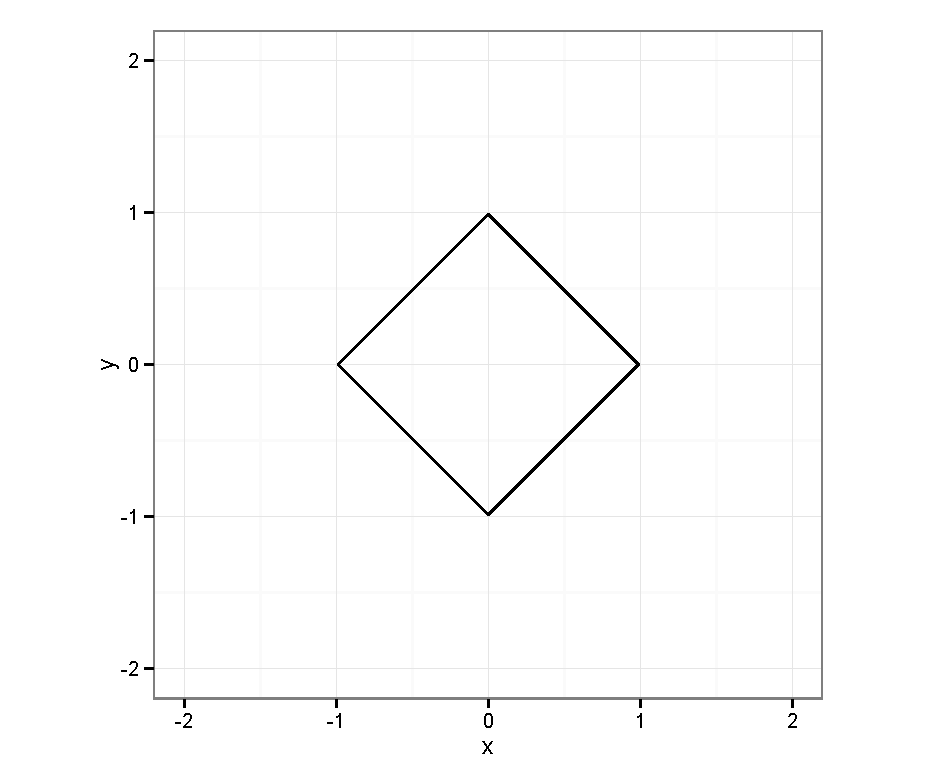
\includegraphics[width=\textwidth]{A_24_A.pdf}
\caption{(i) $p = 1$}
\end{subfigure}
  ~ %add desired spacing between images, e. g. ~, \quad, \qquad, \hfill etc. 
%(or a blank line to force the subfigure onto a new line)
\begin{subfigure}[b]{0.3\textwidth}
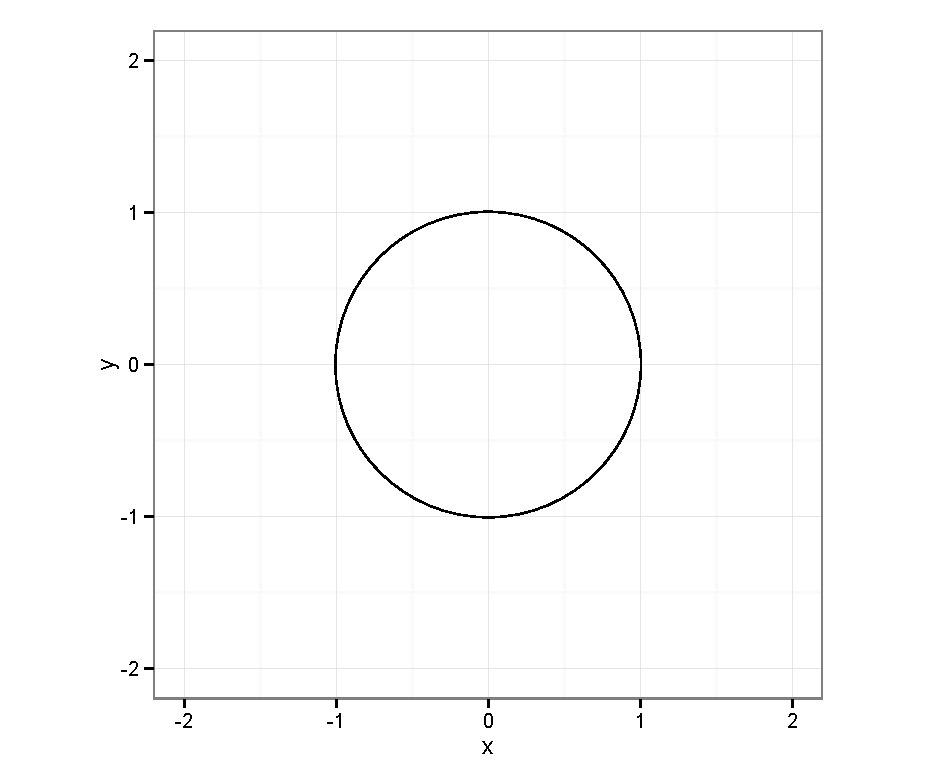
\includegraphics[width=\textwidth]{A_24_B.pdf}
\caption{(ii) $p = 2$}
\end{subfigure}
  ~ %add desired spacing between images, e. g. ~, \quad, \qquad, \hfill etc. 
%(or a blank line to force the subfigure onto a new line)
\begin{subfigure}[b]{0.3\textwidth}
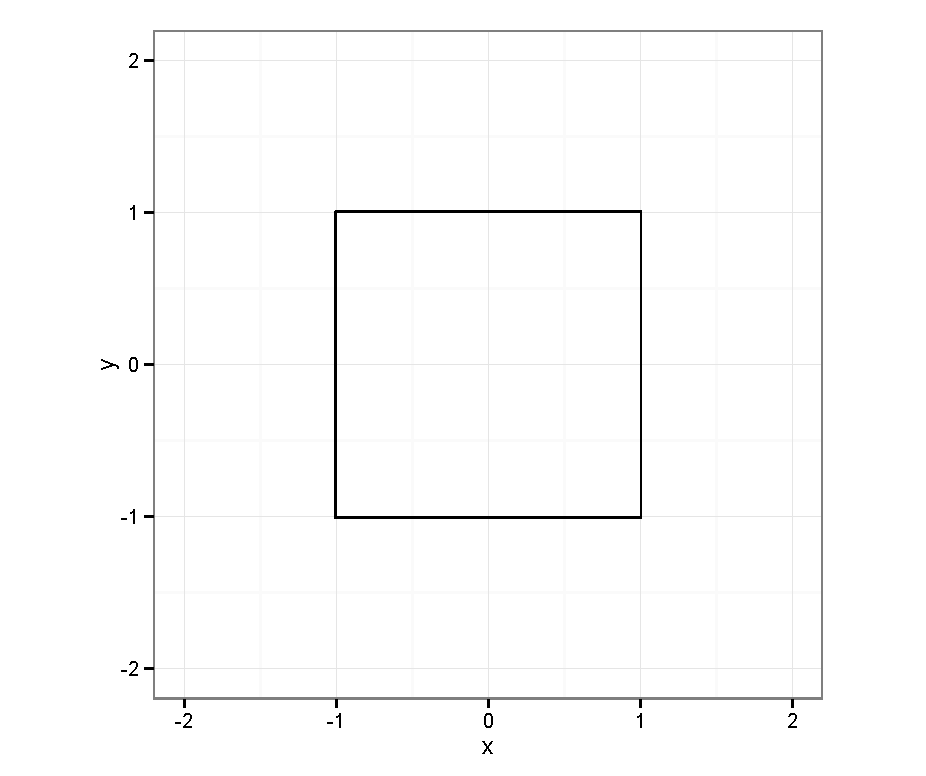
\includegraphics[width=\textwidth]{A_24_C.pdf}
\caption{(iii) $p = \infty$}
\end{subfigure}
\end{figure}


\end{document}

